% L10a weighted majority figure: the weighted vote in each round of the
% lecture's worked example (three experts, four rounds, epsilon = 1/2).
%
% Drawn on October 19, 2026 with the palette and build of the L9c figures.
%
% Each round is a tug of war. Every expert is a block whose width is its weight
% before the round (2 cm per unit weight), placed on the side it predicted:
% down to the left of the center line, up to the right. The heavier side is our
% prediction: the weight voting columns add up each side, with the heavier
% total in bold. The side matching the outcome is shaded, so the blocks on the
% other side are the mistakes; they get a red outline and are half as wide in
% the next round. Values from the lecture's table:
%   round 1: weights (1, 1, 1),        predictions (up, up, down),  outcome up
%   round 2: weights (1, 1, 1/2),      predictions (down, up, up),  outcome down
%   round 3: weights (1, 1/2, 1/4),    predictions (down, up, up),  outcome up
%   round 4: weights (1/2, 1/2, 1/4),  predictions (up, down, up),  outcome up
% Our vote: up, up, down, up, so we are wrong in rounds 2 and 3.
%
% Math uses the standard TeX fonts (no unicode-math), so symbols render as the
% notebook's math shows them.
%
% The notebook SVG carries a dark palette added by theme_svg.py; keep new
% colors in that script's mapping when changing the palette here.
\documentclass[tikz,border=4pt]{standalone}
\usepackage[no-math]{fontspec}
\IfFontExistsTF{Arial}{\setsansfont{Arial}}{\setsansfont{TeX Gyre Heros}}
\renewcommand{\familydefault}{\sfdefault}
\usepackage{amsmath,amssymb}

% Ink, blue, red, and gray match the L9c figures. Red marks mistakes only, so
% no expert is drawn in red, orange, or green.
\definecolor{vnink}{HTML}{202124}
\definecolor{gdblue}{HTML}{0091FF}
\definecolor{gdred}{HTML}{E02020}
\definecolor{gdgray}{HTML}{6D7278}
\definecolor{wapurple}{HTML}{8E5CD9}
\definecolor{waband}{HTML}{EEF0F2}

% \expertblock{left edge}{weight}{row y}{expert}: one expert's vote, 2 cm per
% unit weight, inset so neighboring blocks and their outlines stay distinct.
\newcommand{\expertblock}[4]{%
  \fill[e#4, rounded corners=1.5pt] (#1 + 0.08, #3 - 0.25) rectangle (#1 + 2*#2 - 0.08, #3 + 0.25);
  \node[text=white, font=\sffamily\small\bfseries, text height=1.6ex, text depth=0.45ex] at (#1 + #2, #3) {#4};}
% \wrong{left edge}{weight}{row y}: red outline on a block on the wrong side.
\newcommand{\wrong}[3]{%
  \draw[gdred, line width=1.5pt, rounded corners=2.5pt] (#1 + 0.03, #3 - 0.31) rectangle (#1 + 2*#2 - 0.03, #3 + 0.31);}

\begin{document}
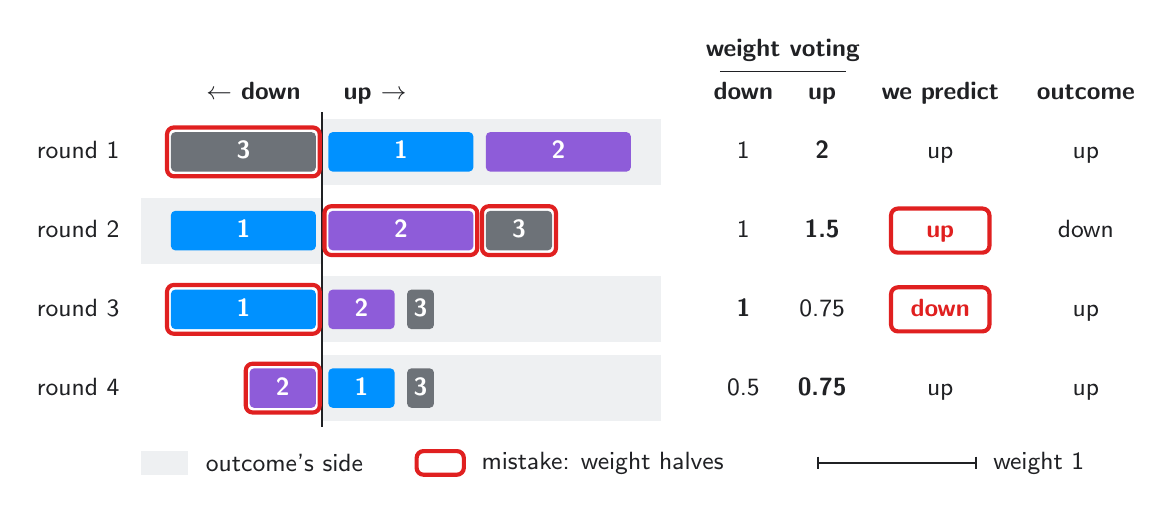
\begin{tikzpicture}[x=1cm, y=1cm, font=\sffamily\small, text=vnink,
    head/.style={font=\sffamily\small\bfseries, text height=1.6ex, text depth=0.45ex},
    cell/.style={text height=1.6ex, text depth=0.45ex},
    pill/.style={cell, minimum width=1.25cm, minimum height=0.56cm, rounded corners=2.5pt, inner sep=0pt},
  ]
  \colorlet{e1}{gdblue}
  \colorlet{e2}{wapurple}
  \colorlet{e3}{gdgray}

  % the outcome's side of each round, drawn first
  \foreach \y/\a/\b in {-1/0/4.3, -2/-2.3/0, -3/0/4.3, -4/0/4.3}
    \fill[waband] (\a, \y - 0.42) rectangle (\b, \y + 0.42);

  % column heads and the center line
  \node[head, anchor=east] at (-0.15, -0.25) {$\leftarrow$ down};
  \node[head, anchor=west] at (0.15, -0.25) {up $\rightarrow$};
  \node[head] at (5.85, 0.3) {weight voting};
  \draw[vnink, line width=0.5pt] (5.05, 0.02) -- (6.65, 0.02);
  \node[head] at (5.35, -0.25) {down};
  \node[head] at (6.35, -0.25) {up};
  \node[head] at (7.85, -0.25) {we predict};
  \node[head] at (9.7, -0.25) {outcome};
  \draw[vnink, line width=0.9pt] (0, -0.5) -- (0, -4.5);

  \foreach \r in {1, 2, 3, 4} \node[cell, anchor=east] at (-2.45, -\r) {round \r};

  % round 1: experts 1 and 2 up (1 + 1), expert 3 down (1); outcome up
  \expertblock{0}{1}{-1}{1} \expertblock{2}{1}{-1}{2} \expertblock{-2}{1}{-1}{3}
  \wrong{-2}{1}{-1}
  % round 2: experts 2 and 3 up (1 + 1/2), expert 1 down (1); outcome down
  \expertblock{0}{1}{-2}{2} \expertblock{2}{0.5}{-2}{3} \expertblock{-2}{1}{-2}{1}
  \wrong{0}{1}{-2} \wrong{2}{0.5}{-2}
  % round 3: experts 2 and 3 up (1/2 + 1/4), expert 1 down (1); outcome up
  \expertblock{0}{0.5}{-3}{2} \expertblock{1}{0.25}{-3}{3} \expertblock{-2}{1}{-3}{1}
  \wrong{-2}{1}{-3}
  % round 4: experts 1 and 3 up (1/2 + 1/4), expert 2 down (1/2); outcome up
  \expertblock{0}{0.5}{-4}{1} \expertblock{1}{0.25}{-4}{3} \expertblock{-1}{0.5}{-4}{2}
  \wrong{-1}{0.5}{-4}

  % each side's total weight; the heavier side, in bold, is our prediction
  \foreach \y/\d/\u in {-1/1/\textbf{2}, -2/1/\textbf{1.5}, -3/\textbf{1}/0.75, -4/0.5/\textbf{0.75}} {
    \node[cell] at (5.35, \y) {\d};
    \node[cell] at (6.35, \y) {\u};
  }

  % our prediction, the heavier side, outlined in red when it is wrong; the outcome
  \foreach \y/\v in {-1/up, -4/up} \node[pill] at (7.85, \y) {\v};
  \foreach \y/\v in {-2/up, -3/down}
    \node[pill, draw=gdred, line width=1.5pt, text=gdred, font=\sffamily\small\bfseries] at (7.85, \y) {\v};
  \foreach \y/\v in {-1/up, -2/down, -3/up, -4/up} \node[cell] at (9.7, \y) {\v};

  % key
  \fill[waband] (-2.3, -5.1) rectangle (-1.7, -4.8);
  \node[anchor=west] at (-1.6, -4.95) {outcome's side};
  \draw[gdred, line width=1.5pt, rounded corners=2.5pt] (1.2, -5.1) rectangle (1.8, -4.8);
  \node[anchor=west] at (1.9, -4.95) {mistake: weight halves};
  \draw[vnink, line width=0.8pt] (6.3, -4.95) -- (8.3, -4.95);
  \foreach \x in {6.3, 8.3} \draw[vnink, line width=0.8pt] (\x, -4.87) -- (\x, -5.03);
  \node[anchor=west] at (8.4, -4.95) {weight 1};
\end{tikzpicture}
\end{document}
